Visualization features are dependant on the imaging acquisiton process.
In this preprocessing step, the user performing the imaging acquistion has to decide on two critical visualization components.
\\ First, the user needs to decide which patient specific tissues are relevant to the procedure, i.e. arteries, bone, skin, and segment them.
Then, the material which decides how the 3D model will be rendered in the engine (i.e. Unity3D), needs to be set.
These segment specific materials can be given a color in such a way that visualization is improved, i.e. highlight specific critical tissue.
By setting the alpha value of the materials lower than one, segments can be set to be transparent.
\\ Second, the user has to decide on the resolution of the 3D models segments, meaning the number of polygons which represent the model.
This is especially important when factoring in the VR-AR-based workflow, in which the AR glasses capabilities limit the resolution of the model.
The user has to strike a balance between system performance and resolution of the model, but the resolution of the model still has to be high enough so that patient data is displayed realistically.

\begin{figure}[ht]
  \centering
  \begin{minipage}{.5\textwidth}
    \centering
    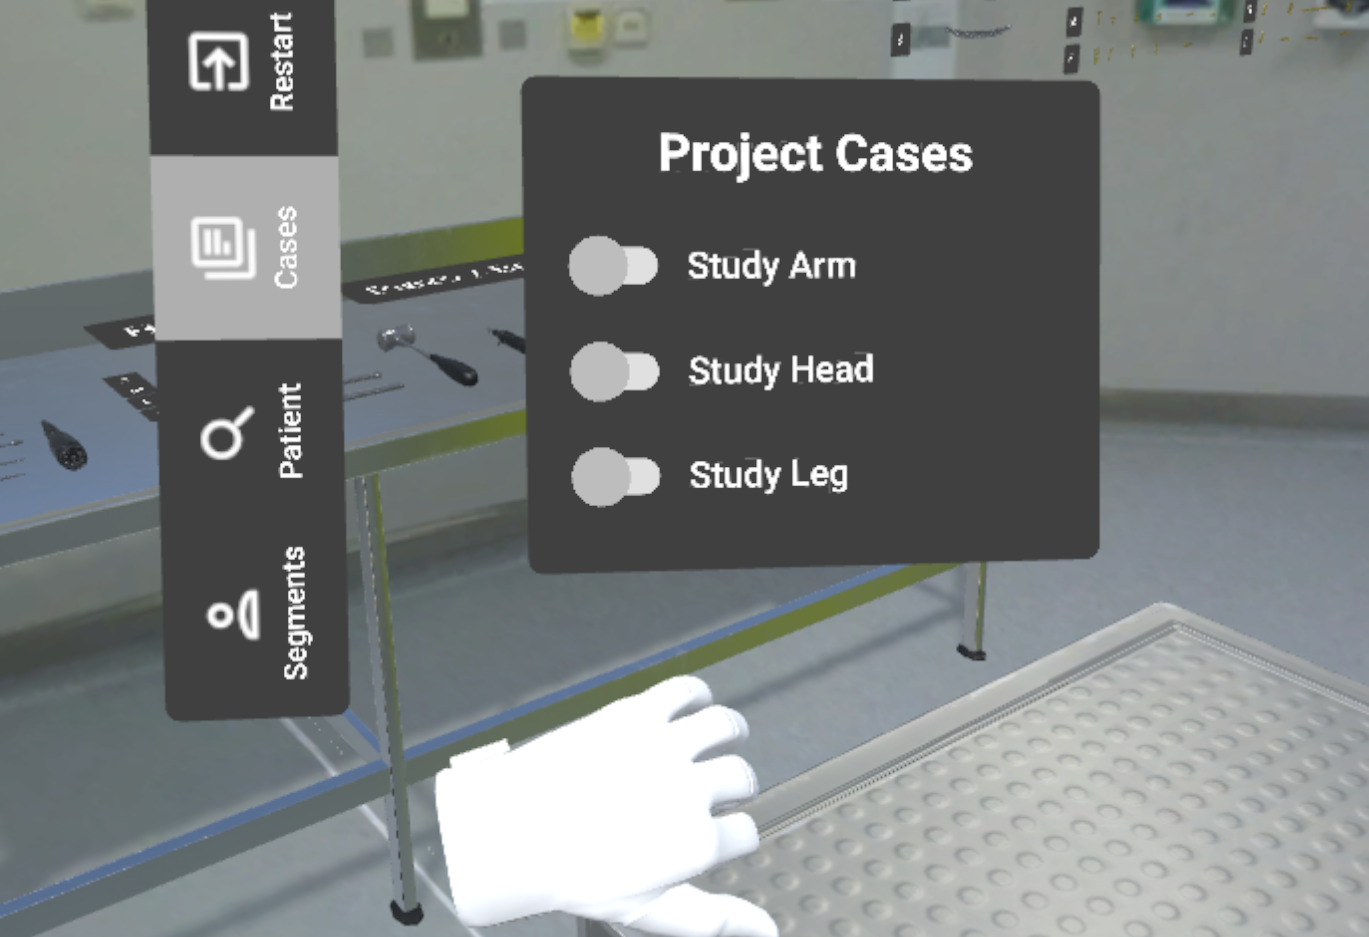
\includegraphics[width=0.99\linewidth]{images/implementation/user_interface/project_case_pre_load.png}
  \end{minipage}%
  \begin{minipage}{.5\textwidth}
    \centering
    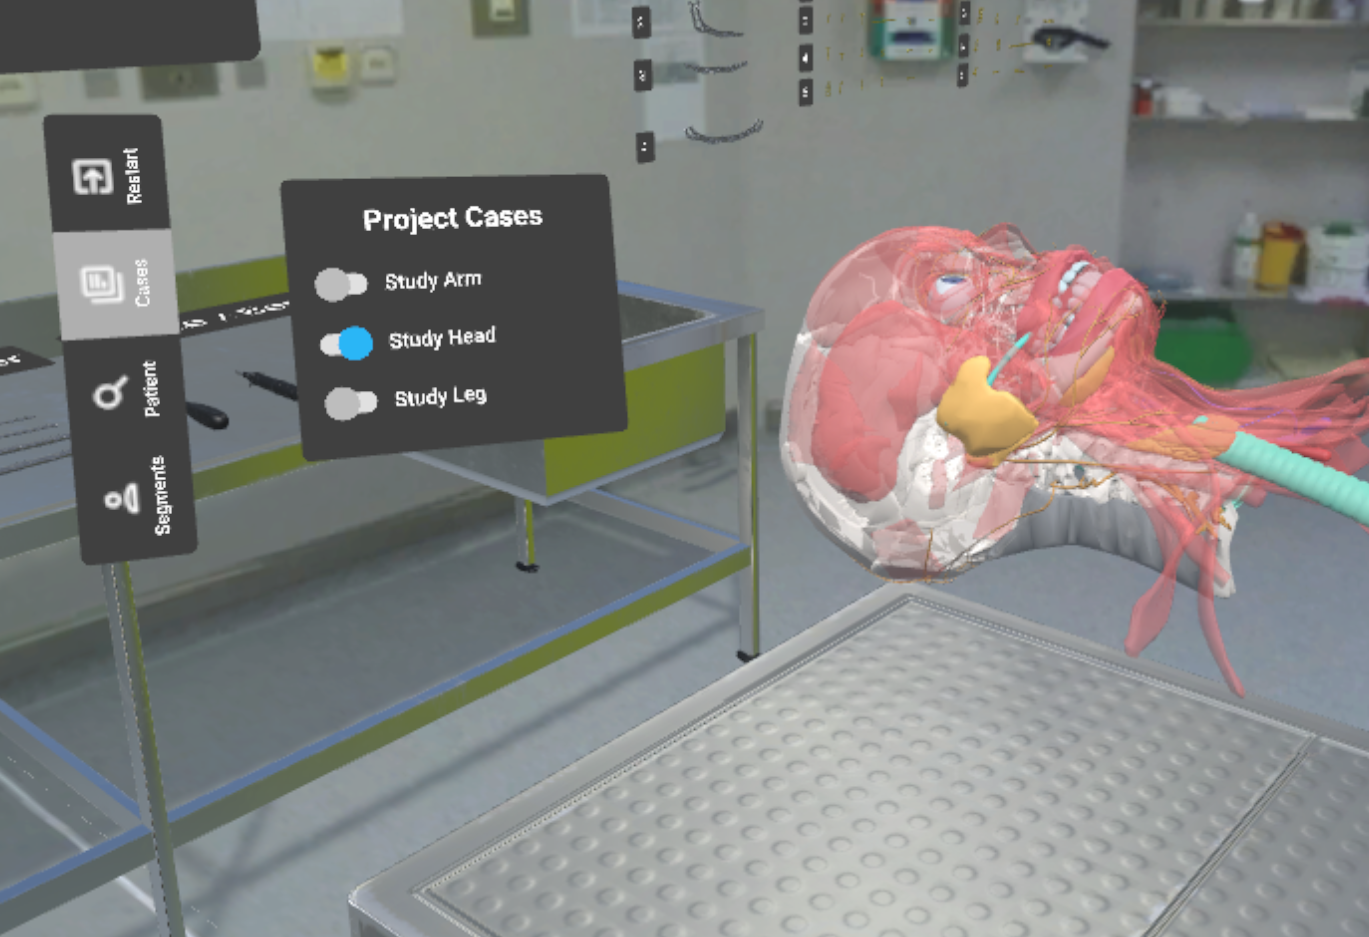
\includegraphics[width=0.99\linewidth]{images/implementation/user_interface/project_case_loaded.png}
  \end{minipage}
  \caption{\label{fig::LoadingProjectCase} Left: The user is about to start working on a project case and presses the B button to view the GUI. Right: The user has selected the "Study head" case and the patient model is loaded into the virtual OT.}
\end{figure}

After finishing this crucial preprocessing step, the file location of the model must be registered in the project case.
Importing models into the VR application is realized through loading a project case via the GUI (Figure \ref{fig::LoadingProjectCase}).
For this application, the data format Wavefront OBJ (OBJ) for 3D geometric data was chosen \cite{WavefrontOBJ}.
OBJ was chosen because of the relatively easy serialization of the 3D data via text as well as its open-source nature. 
Loading of the project case depends on the resolution of the imported model, since the import happens at run-time and is realized through a custom OBJ importer. 

\begin{figure}[ht]
  \centering
  \begin{minipage}{.5\textwidth}
    \centering
    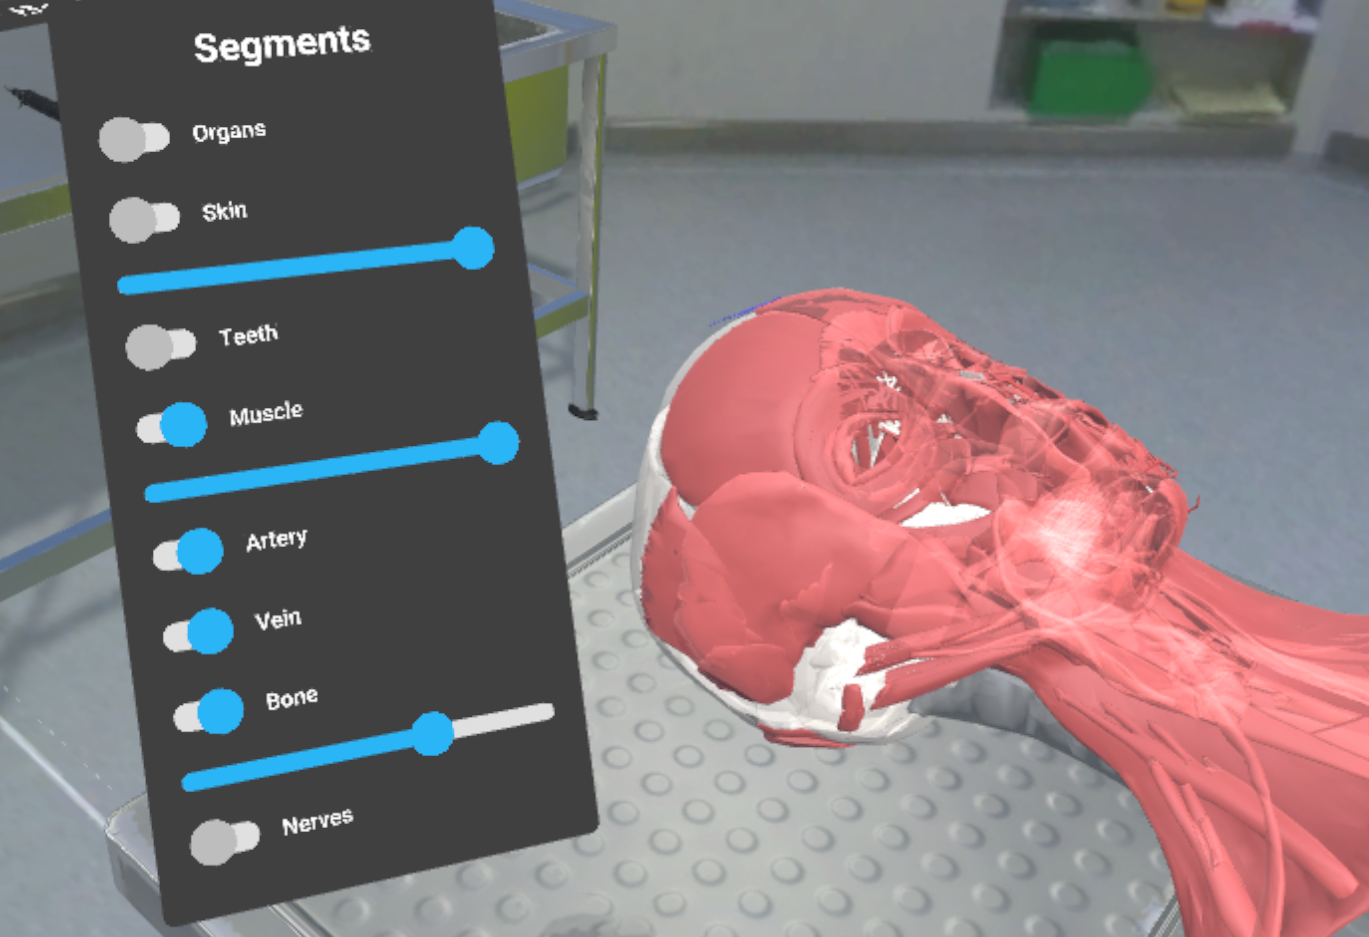
\includegraphics[width=0.99\linewidth]{images/implementation/features/visualization/segments_1.png}
  \end{minipage}%
  \begin{minipage}{.5\textwidth}
    \centering
    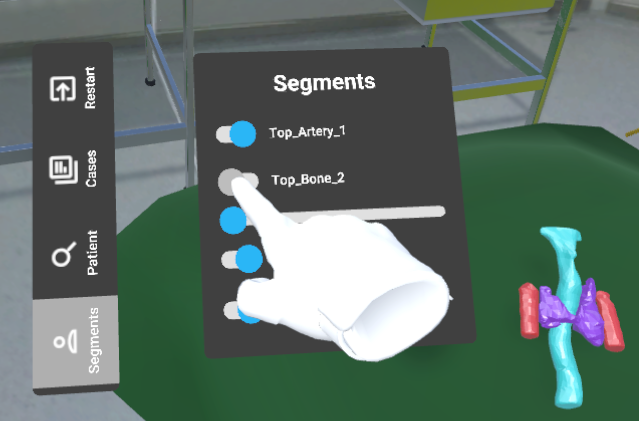
\includegraphics[width=0.99\linewidth]{images/implementation/features/visualization/segments_2.png}
  \end{minipage}
  \caption{\label{fig::Segmentation}Segment submenu of the GUI. Segments are toggled on and off by pressing the button with the virtual hand. Muscle tissue has been toggled off to get a better view on the underlying pathalogy of the patient.}
\end{figure}

In Figure \ref{fig::Segmentation}, the process of activating and deactivating specific segments is described.
Initially, all segments of the loaded patients model will be toggled on.
This is indicated by the blue color and the orientation to the right of the UI element.
Individual segments can be toggled on and off by pressing the virtual button as described in Section \ref{sec::GraphicalUserInterface}.
The GUI will indicate whether a segment is toggled on or off as depicted in Figure \ref{fig::Segmentation}.
Segments which are toggled off are indicated by the gray color and the orientation to the left of the UI element.
Users can also decide to adjust the transparency of segments as desired.
The transparency slider sets the alpha value for the opacity of the segment‘s material to a value between 0 and 1.
The slider is used by holding a finger on it and dragging it to the desired value.

\begin{figure}[ht]
  \centering
  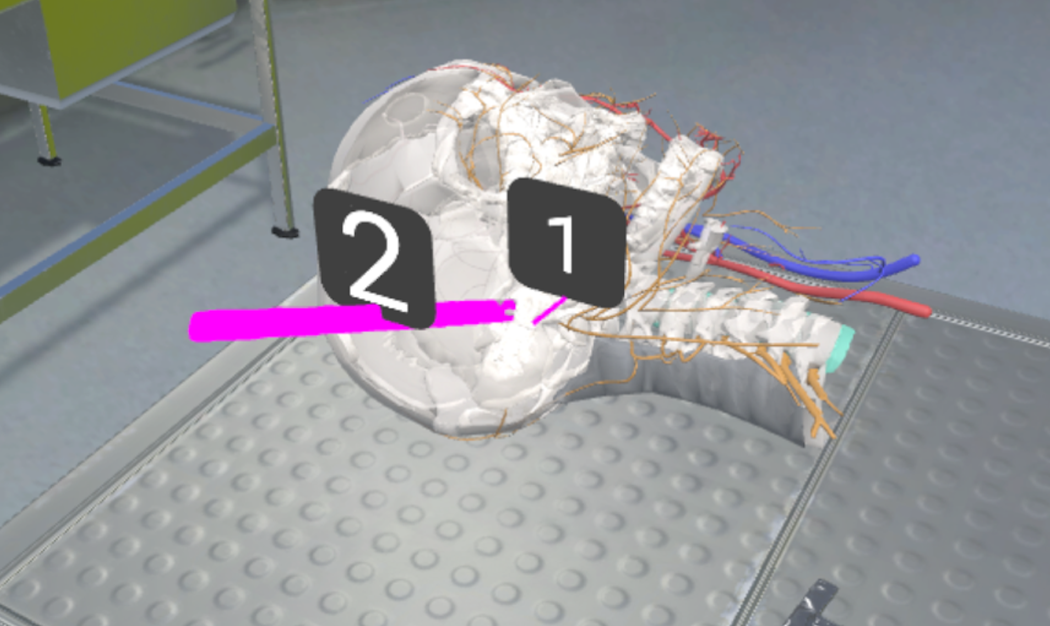
\includegraphics[width=\linewidth]{images/implementation/features/visualization/show_all.png}
  \caption{\label{fig::ShowAll}Patients can invoke the show all command of the VUI at any time to get an overview of the current procedure. Procedure steps are enumerated so that the sequence of the procedure can be followed.}
\end{figure}

To get a complete overview of the planned procedure it is possible to use the voice command "show all" to get a numbered overview of all procedure steps as depicted in Figure 3. 
This way users can prepare themselves for the procedure, e.g. by putting the necessary instruments together on the operating table.

\begin{figure}[ht]
  \centering
  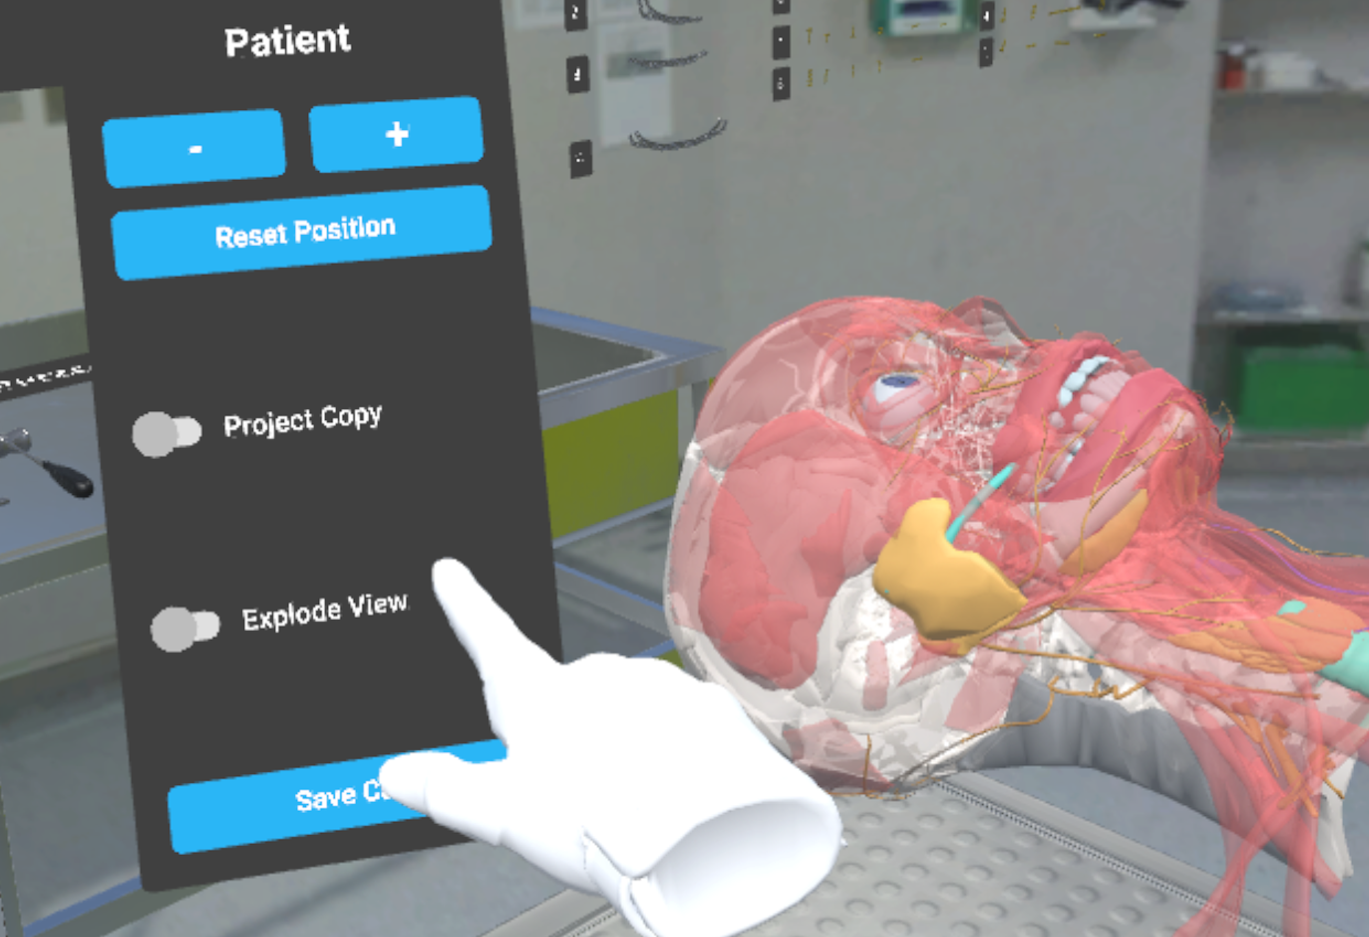
\includegraphics[width=\linewidth]{images/implementation/user_interface/patient_submenu.png}
  \caption{\label{fig::PatientVisualization}Patient submenu of the GUI. Users can scale patients and reset the scale and position to the default. Additional options such as projecting a 
  copy of the patient model or an explode view can be toggled on and off here. The current procedure can also be saved here.}
\end{figure}

In the \emph{Patient} submenu of the GUI additional visualization tools which are not patient specific are located.
Here, the whole virtual patient can be scaled up or down via their respective button (Figure \ref{fig::PatientVisualization}).
Since procedure steps are subcomponents of the virtual patient, done procedures are also scaled correctly and relative spatial relationships can be investigated.
At any time, users can reset the scale, position and rotation of the patient's 3D model to their defaults.
The currently planned procedure can also be saved at any point here by pressing the button at the bottom (Requirement \ref{req::F6}).
Saving the current procedure will persist the current patient model to the users hard disk without overwriting the initial model.
Serialization of the model is realized through a custom runtime OBJ exporter, which writes the models representation, including materials, to a text file.

\begin{figure}[ht]
  \centering
  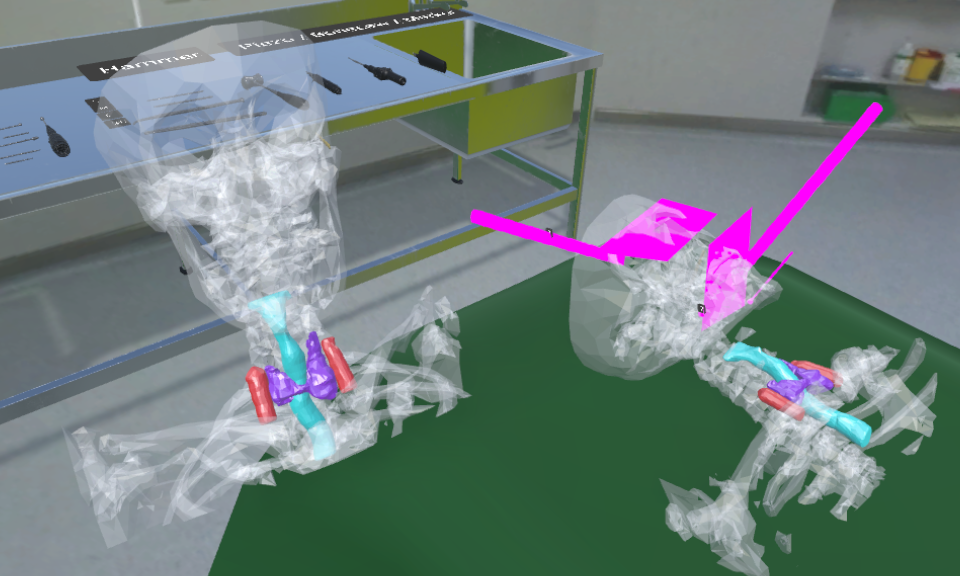
\includegraphics[width=\linewidth]{images/implementation/features/visualization/project_copy.png}
  \caption{\label{fig::ProjectCopy} Projected copy of the unmodified patient model. Users can interact with the copy by grabbing it.}
\end{figure}

Additionally, by pressing the respective button, the user can project a copy of the unmodified patient's model in front of himself at any time, without any procedure steps, for comparison as 
depicted in Figure \ref{fig::ProjectCopy}.
In contrast to the heavily modified patient model to the right, the initial patient model is used to visualize the patient specific anatomy and pathology without any 
friction (Requirement \ref{req::F3.2}).
The projected copy is a literal copy of the loaded patient's model which is created simultaneously when loading a project case.
Users can also interact with the projected copy, meaning they can move and rotate it by grabbing it.

\begin{figure}[ht]
  \centering
  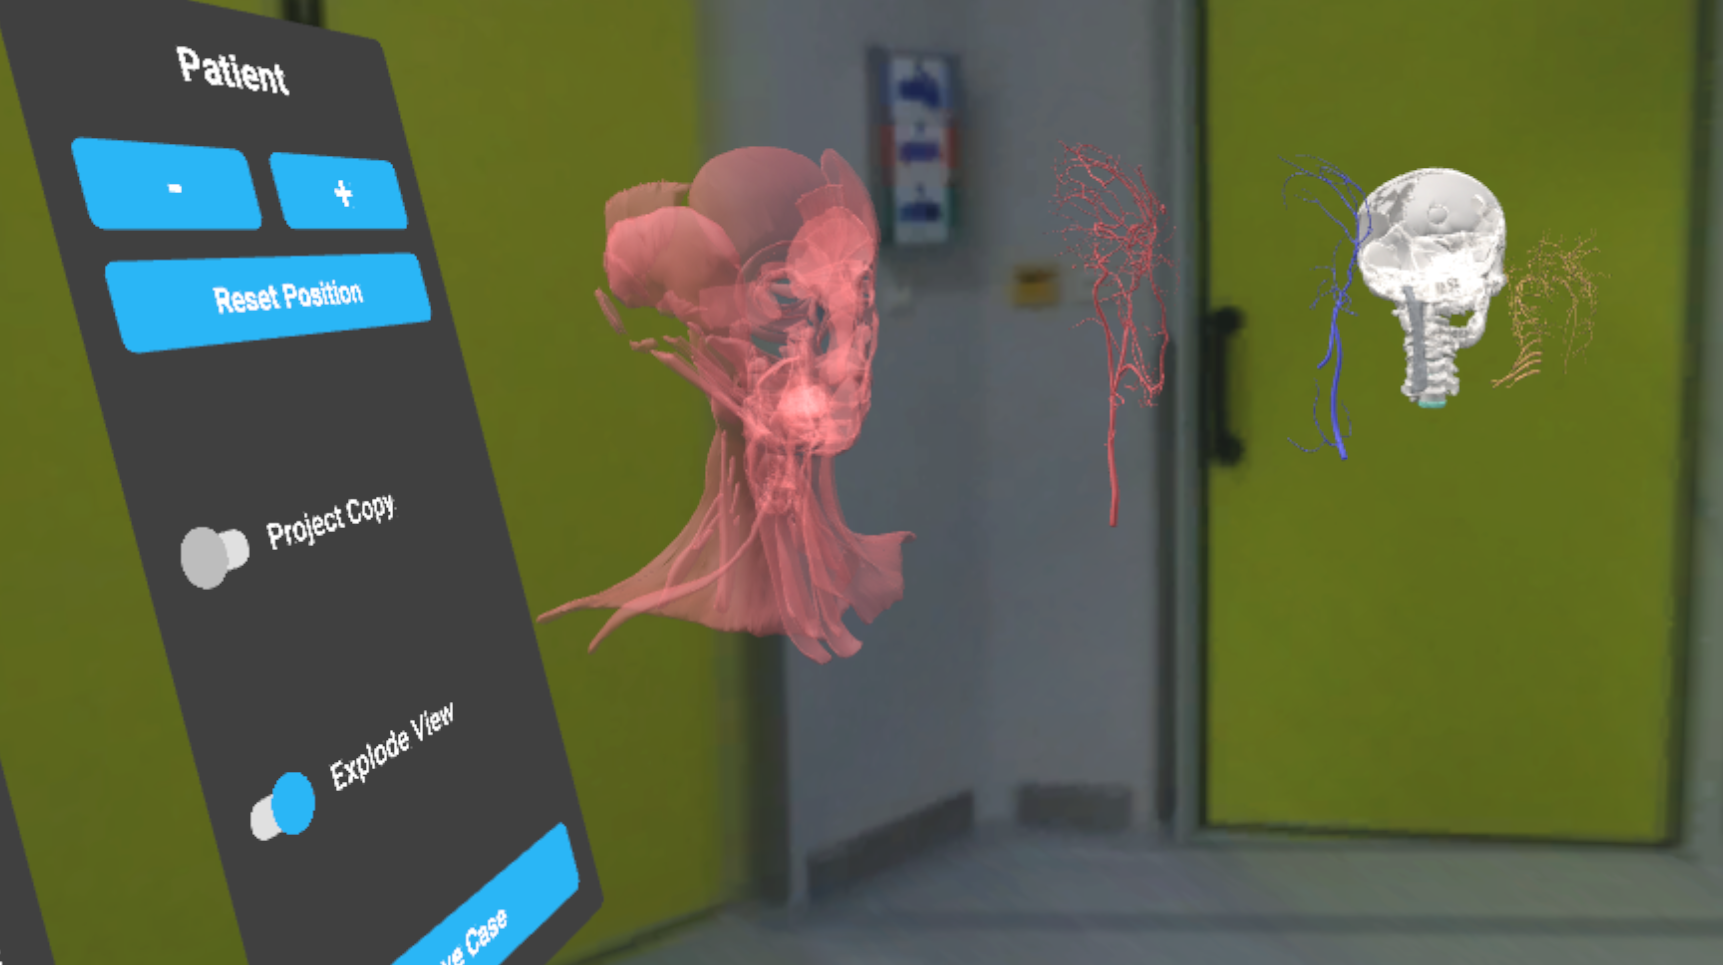
\includegraphics[width=\linewidth]{images/implementation/features/visualization/explode_view.png}
  \caption{\label{fig::ExplodeView} Exploded view of the segments. Here, individual segments are interactable, meaning the rotation and location can be adjusted.}
\end{figure}

The main model of the patient can also be exploded as depicted in Figure \ref{fig::ExplodeView}.
Segments are exploded in a way to allow for individual inspection.
The explode view starts at a specified point in the operating room and each segment is then seperated by a specified distance.
Each segment in the explode view is interactible in such a way that they can be rotated and translated by grabbing it (Requirement \ref{req::F3.3}).

\begin{figure}[ht]
    \centering
    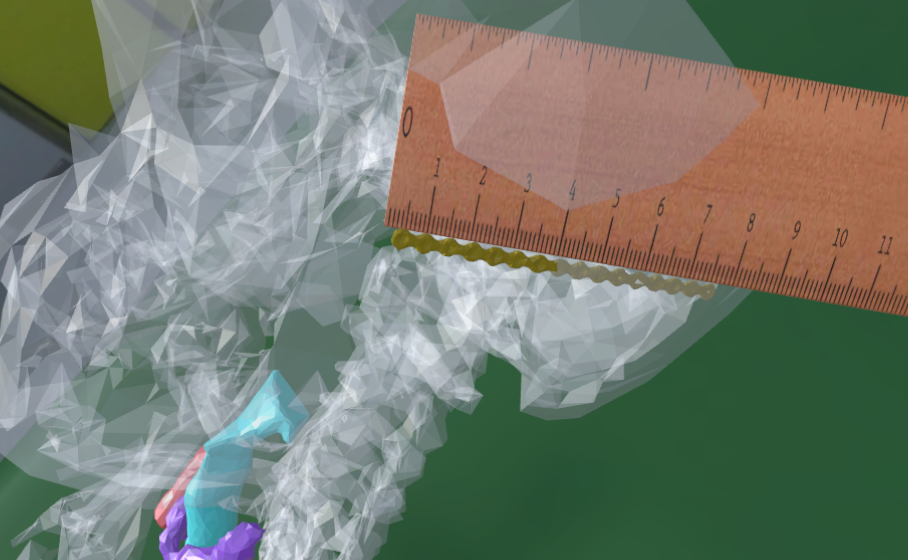
\includegraphics[width=\linewidth]{images/implementation/features/visualization/ruler.png}
    \caption{\label{fig::FeatureRuler} Ruler for checking relative distances. Spatial relationships between tissue are inspected here.}
\end{figure}

In the virtual operating room, a ruler can be used to measure distances, but more importantly relative distances in the patients morphology.
The ruler can simply be picked up via a grab gesture and used in the same way a surgeon uses it.